\section{Evaluation of Surrogate Contact Model}
\label{sec:scm_evaluation}

\rev{This section validates the fidelity of SCM before system-level experiments.} SCM replaces the dense Delassus matrix $\boldsymbol{W}_{\text{env}}$ by its block-diagonal approximation and evaluates $\boldsymbol{\hat{\lambda}}_{\text{env}}$ in closed form under Assumptions~\ref{assumption:mode}--\ref{assumption:decoupling}. We verify that the resulting one-step prediction error against higher-fidelity models is small, and that occasional large single-step gaps do not prevent task success when the CSO-optimal force is applied directly.

We use the fingertip ground-rotation setup with the same $h=0.02$\,s, $\boldsymbol{M}_o$, and success condition~\eqref{eq:pose_success} as below. At each step, CSO selects the optimal candidate $\boldsymbol{\hat{p}}^*_{\text{r}}\in\mathcal{I}_{\text{avail}}$ and its best force $\boldsymbol{\hat{\lambda}}^*_{\text{r}}$, and SCM predicts $\boldsymbol{\hat{v}}^+$ and $\boldsymbol{\hat{\lambda}}_{\text{env}}$. Under identical free velocity $\boldsymbol{v}_{\text{free}}$, environment Jacobian $\boldsymbol{\tilde{J}}_{\text{env}}$, and $\boldsymbol{M}_o^{-1}$, we compute the rigid-pyramid LCP reference via Lemke's algorithm and a MuJoCo QP reference via a single \texttt{mj\_forward}. Following Lemma~\ref{lem:scm_accuracy} and Appendix~\ref{app:scm_motion_accuracy}, we report the inertia-weighted direction error $\theta$ with $\cos\theta_{M_o}$, the magnitude gap $\big|\|\boldsymbol{v}^+\|_{\boldsymbol{M}_o}-\|\boldsymbol{\hat{v}}^+\|_{\boldsymbol{M}_o}\big|$, and the multiplier gap $\|\boldsymbol{\hat{\lambda}}_{\text{env}}-\boldsymbol{\lambda}_{\text{env}}\|_{\boldsymbol{D}}$. Each rollout then directly applies the CSO-optimal contact by tracking the predicted orientation and the goal-directed component of the predicted translation, without CPO or OSC.

Table~\ref{tab:scm_eval} summarizes the results over repeated ContactDB objects. Against LCP, the median direction error is around $0.19$\,rad with magnitude and multiplier gaps at the $10^{-3}$--$10^{-2}$ scale; larger gaps concentrate on a few contact-set transition steps. The MuJoCo single-step gap is occasionally larger due to its full-body contact resolution, but the goal-directed motion trend is preserved. Every direct-apply trajectory satisfies~\eqref{eq:pose_success} within $160$ steps, indicating that SCM preserves the contact-selection signal needed by CSO.

\begin{table}[t]
\centering
\caption{Fidelity of SCM against the rigid LCP and success of direct-apply rollouts.}
\label{tab:scm_eval}
\begin{tabular}{lcccc}
\toprule
\textbf{Metric} & \textbf{Success} & \textbf{dir $\theta$} (rad) & \textbf{mag.\ gap} & \textbf{$\|d\boldsymbol{\lambda}\|_{\boldsymbol{D}}$} \\
\midrule
SCM vs.\ LCP (median) & --- & $0.19$ & $0.005$ & $0.05$ \\
SCM vs.\ LCP (mean) & --- & $0.33$ & $0.029$ & $0.069$ \\
Direct-apply rollout & $100\%$ & --- & --- & --- \\
\bottomrule
\end{tabular}
\end{table}

\section{Experiment: Nonprehensile Manipulation}
\label{sec:experiment}

\rev{This section evaluates the SCSP framework through experiments.} We first conduct nonprehensile manipulation experiments, which represent a complex contact-rich manipulation task with high demands on operational diversity and control robustness. The task is to adjust the pose of an object on the ground through nonprehensile manipulation, which consists of:
\begin{itemize}
    \item \textbf{On-ground rotation:} The robot needs to move the object to the target pose on the ground through pushing and rotating, which constitutes a 2D planar pushing task.
    \item \textbf{On-ground flipping:} The robot needs to move the object to the target pose on the ground through pushing and flipping, which constitutes a 6D manipulation task.
\end{itemize}
We select a set of complex-shaped objects from the ContactDB dataset \cite{brahmbhatt2019contactdb} for validation. The objects are initialized at random poses with 
$x_{\text{init}}, y_{\text{init}} \in [-0.3, 0.3]$ m, 
and Euler angles $(\phi_{\text{init}}, \theta_{\text{init}} , \psi_{\text{init}})$ 
uniformly sampled from $[-\pi, \pi]$ rad. We define the conditions of task success as: 
\begin{equation}
    \left\| \boldsymbol{p}_o - \boldsymbol{p}_{\text{goal}} \right\|
\le 0.02 \,\text{[m]}, \ 
1 - (\boldsymbol{\psi}_{\text{goal}}^\top \boldsymbol{\psi}_o)^2
\le \textcolor{red}{0.015}, \label{eq:pose_success}
\end{equation}
\textcolor{red}{where the orientation tolerance corresponding to the quaternion error threshold is approximately $14.1^\circ$.} A trial is considered successful if the conditions are satisfied within 2500 rollout steps. We evaluate the algorithm on different robot platforms, namely a fingertip\footnote{The ``fingertip'' is a floating point with a collision volume and is commonly used as a simplified setup for validating contact planning methods.} and the Franka Emika Panda, and compare different methods in terms of success rate, efficiency, and convergence error. \rev{These experiments evaluate whether SCSP can select contact locations and complete tasks under complex contact interactions.} 

Simulations are conducted in \texttt{MuJoCo} \cite{todorov2012mujoco} and  \texttt{IsaacGym} \cite{makoviychuk2021isaac} with a fixed integration time step $h=0.02 \text{s}$. For the sampling method in our CSO module, we use \texttt{CoACD} \cite{wei2022approximate} for convex decomposition of the objects and \texttt{trimesh} for mesh processing and local frame construction. The inner loop of CSO is implemented by solving the nonlinear SQP optimization using \texttt{CasADi} \cite{Andersson2019} with \texttt{SNOPT} \cite{gill2005snopt} solver, and the solver of CPO is \texttt{IPOPT} \cite{wachter2006implementation}. \rev{All experiments are conducted} on a desktop computer with the Intel i7-13620H processor and 32 GB RAM.

We applied certain randomization to the environment and object parameters. The friction coefficients of the object $\mu_{\text{o}}$, fingertip $\mu_{\text{r}}$, and ground $\mu_{\text{env}}$ are all set to 0.5 with random perturbations of $\pm 0.2$. The object mass is set to $0.1$ kg and randomly sampled from the discrete set
$\{0.01,0.1,1.0,10.0\}$ kg. We set $\boldsymbol{M}_o=\text{diag}(50,50,50,0.05,0.05,0.05)$ and $\boldsymbol{K}_r=300 \boldsymbol{I}_7$, and the dynamic parameters used in SCM are not measured precisely, but are instead roughly set to their mean values. For CSO, we set $n_s=70$ and $\hat{\lambda}^n_{\text{max}}=0.2$. For CPO, we set $\bar{\rho}=0.75$, $T_1=5$, $T_2=10$, $T_3=15$, $\varepsilon=0.01$, $w_{\text{lp}}=1$, $w_{\text{pos}}=500$, $w_{\text{quat}}=5$, $w_\text{u}=50$, $w_{\text{obj}}=10$. We conducted parameter tuning via grid search over 100 randomly sampled trials, and the resulting parameters were fixed for all subsequent experiments. In addition, based on the definition of the object’s local coordinate frame and the planar environment in the experiments, the stable pose set $\mathcal{X}_g$ can be written as $\mathcal{X}_g=\left\{\boldsymbol{x}_o\in\mathcal{X}\;\middle|\;\boldsymbol{R}\left(\boldsymbol{x}_o\right)e_z=e_z\right\}
$ with $e_z=[0, 0, 1]^\top$. Therefore, $\ell_{\text{stab}}$ is defined as:
\begin{equation}
    \ell_{\text{stab}}=1-\bigl(\boldsymbol{R}(\boldsymbol{x}_o)e_z\bigr)^\top\bigl(\boldsymbol{R}(\boldsymbol{x}_{\text{goal}})e_z\bigr).
\end{equation}

From Table \ref{tab:comparison}, we select the methods that are applicable to 6D manipulation, operate in real time, and can handle arbitrary manipulable object geometries as baselines, including:
\begin{itemize}
    \item \textbf{DyWA} \cite{lyu2025dywa}:  An end-to-end 6D nonprehensile manipulation with generalization across diverse unseen objects. We follow the settings in their released source code by adding the test objects to the \texttt{IsaacGym}, and evaluate the performance of the single-view student policy. 
    \item \textbf{Sampling} \cite{venkatesh2025approximating}: A class of hierarchical frameworks  in which the upper layer selects a set of candidate contact points by sampling on the object envelope. The upper layer performs contact selection by evaluating the CIMPC cost and control cost in parallel, while the lower layer uses OSC to achieve approach and contact. To eliminate the effect of differences in contact modeling, we replace the original C3 model \cite{aydinoglu2024consensus} in \cite{venkatesh2025approximating} with $f_{\text{cf}}$.
    \item \textbf{I-MPC:} A CIMPC method based on a QP-based contact model. This method performs contact simulation by solving the KKT conditions of the contact model and implicitly plans the contact mode, force, and location by optimizing robot-centric control inputs. The stage cost is defined as the sum of a contact cost and a control cost $\ell = \left \| \boldsymbol{p}_{\text{obj}} - \boldsymbol{p}_{\text{ee}} \right \|^2 +\left \| \boldsymbol{u} \right \|^2$
and the terminal cost is defined the same as \eqref{equ:obj_pose_cost}. Although the contact planning formulation is unified and does not use hierarchical solving for different contact modes, the planning horizon is short to enable online computation. In addition, the method relies on explicitly defined contact costs to encourage robot–object interaction. As a result, it can only adjust the contact location to a  limited extent.
    \item \textbf{CF-MPC} \cite{jin2024complementarity}: A complementarity-free MPC method based on closed-form contact model \eqref{equ:cf_model}. The cost design is the same as in I-MPC, but it uses an improved contact model, achieving higher manipulation success rates and better computational efficiency. However, its underlying formulation remains unchanged, so its contact selection capability is still limited.
    \item \textbf{A-MPC:} We augment CF-MPC by adding an additional alignment cost into the stage cost:
\begin{equation}
\ell_{\text{align}}
=
-\frac{(  \vec{\mathbf{v}} _{\text{obj}}^\text{goal} )^\top
\vec{\mathbf{v}} _{\text{ee}}^\text{obj} + 1}{2},
\end{equation}
in which:
$
\vec{\mathbf{v}} _{\text{obj}}^\text{goal}=\frac{\boldsymbol{p}_{\text{goal}} - \boldsymbol{p}_{\text{obj}}}{\left \| \boldsymbol{p}_{\text{goal}} - \boldsymbol{p}_{\text{obj}} \right \| }, \ 
\vec{\mathbf{v}} _{\text{ee}}^\text{obj}=\frac{\boldsymbol{p}_{\text{obj}} - \boldsymbol{p}_{\text{ee}}}{\left \| \boldsymbol{p}_{\text{obj}} - \boldsymbol{p}_{\text{ee}} \right \| }
$.
 This cost is motivated by a simple intuition: when pushing an object toward a given direction, the optimal contact location often lies on the side opposite to the pushing direction, since the surface is more likely to contain the desired force within the friction cones. Although this heuristic may not hold for objects with complex geometries, it serves as a simple prior that can guide contact planning methods to escape local minima.
    \item \textbf{w/o RS:} A variant of SCSP without the Ranking Strategy in CPO. In this method, CSO and CPO are fully connected, which means that CPO completely follows and executes the contact locations predicted by CSO. This ablation demonstrates that the ranking strategy is a crucial factor for the robustness of SCSP. 
\end{itemize}

\subsection{Fingertip Manipulation in Simulation}\label{sec:fingertip_exps}

We first conduct fingertip manipulation to validate the critical role of contact selection in contact-rich manipulation. Since DyWA is an offline-trained policy, it is not applicable to the fingertip experiments and is therefore omitted. By comparing with other model-based methods, we demonstrate that explicitly introducing a contact selection module is effective for handling complex manipulation tasks. 




\begin{figure}[!t]
 \centerline{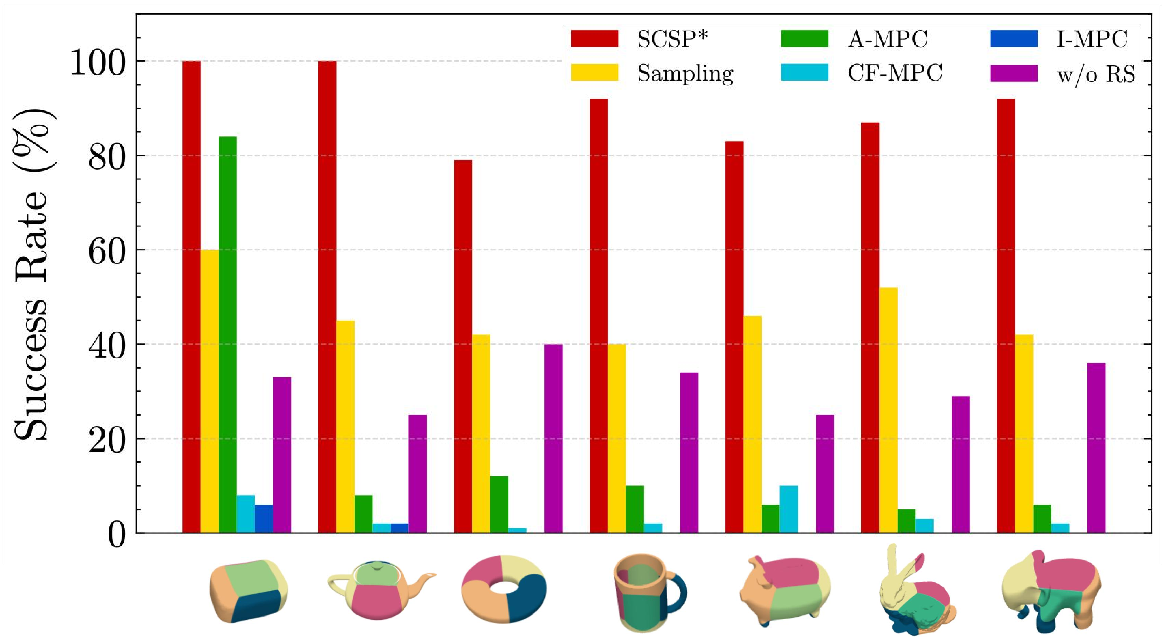
\includegraphics[width=\columnwidth]{figures/fingertip_exp.pdf}}
\caption{Experimental results of fingertip manipulation. SCSP achieves a substantially higher success rate than the other methods.}
\label{fig:results_fingertip}
\end{figure}


The experimental results are shown in Fig. \ref{fig:results_fingertip}, \ref{fig:simulation_data} and Table \ref{tab:all_data}. Compared with the baseline methods, SCSP achieves a significantly higher success rate, shorter execution time, and lower final position and quaternion errors. Our observations indicate that most of the successful cases of I-MPC and CF-MPC correspond to a good robot initial state, where the methods can succeed by applying contact forces at a fixed contact location. When the fingertip initial position is poor, they exhibit almost no adjustment capability. A-MPC achieves a significant improvement in success rate, demonstrating that even a coarse contact selection prior can substantially mitigate the local optimum problem in contact planning. Sampling achieves further improvement but at the cost of lower computational efficiency. These experimental results highlight the importance of active contact selection in complex tasks.

\subsection{Robot Manipulation in Simulation}\label{sec:robot_manipulation}

We further evaluate SCSP in redundant robot manipulation tasks. Compared with floating-based fingertip, contact problems for redundant robots introduce complex kinematic constraints. In the experiments, we demonstrate the superiority of SCSP and validate the soundness of our framework.



\begin{figure}[!t]
 \centerline{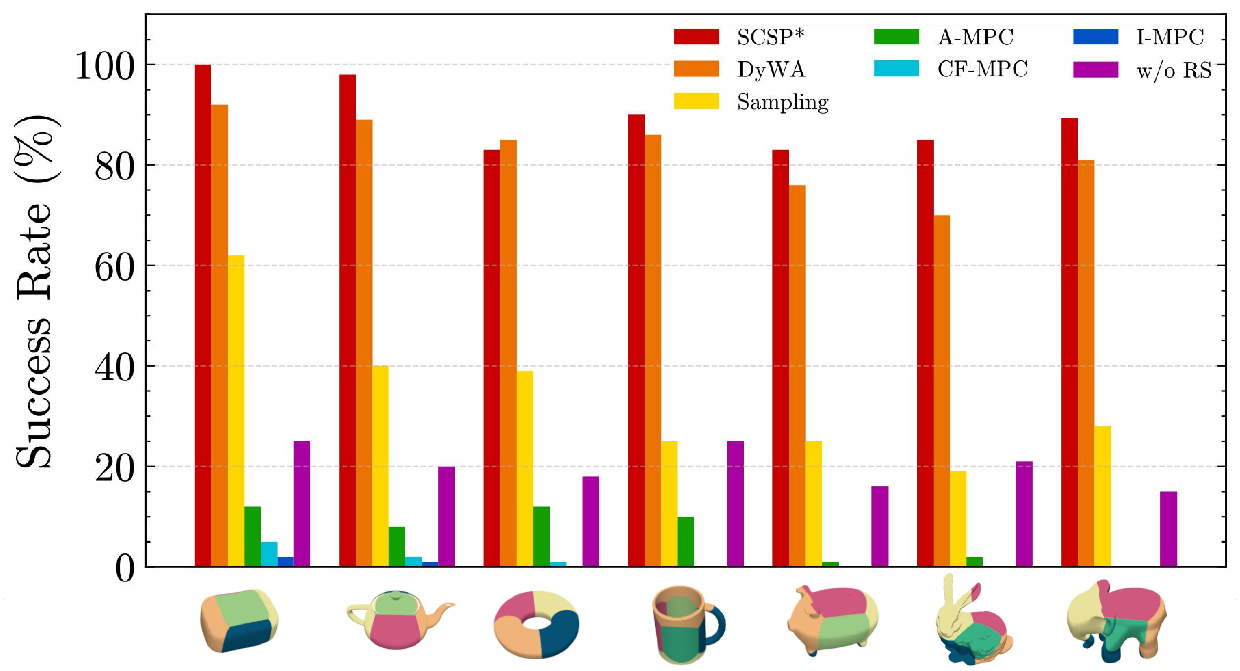
\includegraphics[width=\columnwidth]{figures/franka_exp.pdf}}
\caption{Experimental results of robot manipulation in simulation. SCSP significantly outperforms other model-based methods and exceeds the performance of well-trained learning-based methods.}
\label{fig:results_panda}
\end{figure}

Due to the strong dependencies of the source code released for DyWA, which are difficult to transfer, we follow its setup and conduct all experiments in \texttt{IsaacGym} for consistency, with other settings similar to Section \ref{sec:fingertip_exps}. All methods use our link-mounted sphere as the end-effector to replicate point contacts. Since DyWA uses the Franka gripper, we adjust the link length so that the sphere’s center coincides with the gripper’s center. The Cartesian stiffness $\boldsymbol{K}_x=\text{diag}(1000,1000,1000,50,50,50)$ and $\boldsymbol{D}_x=\sqrt{2\boldsymbol{K}_x}$. All methods use the same settings as in the fingertip experiments, except that $\boldsymbol{u} \in \mathbb{R}^7$ in I-MPC, CF-MPC and A-MPC. $\boldsymbol{p}_{\text{ee}}$ is obtained via differentiable forward kinematics.


\begin{table*}[t]
  \begin{center}
  \caption{
  {Comparison of nonprehensile manipulation tasks of the fingertip experiment and the robot experiment (200 trials).}
}
 \label{tab:all_data}
  
  \resizebox{\linewidth}{!}{
  \begin{tabular}{c|c|cc|cc|cc|cc|cc}
    \toprule[1pt]
    \multirow{2}{*}{\textbf{Platform}}
    & \multirow{2}{*}{\textbf{Method}}
    & \multicolumn{2}{c|}{\textbf{Success Rate}}
    & \multicolumn{2}{c|}{\textbf{Execution Time} (s)}
    & \multicolumn{2}{c|}{\textbf{Planning Time} (s)}
    & \multicolumn{2}{c|}{\textbf{Obj. Pos. Error} (m)}
    & \multicolumn{2}{c}{\textbf{Obj. Quat. Error}} \\

    \cmidrule(lr){3-4} \cmidrule(lr){5-6} \cmidrule(lr){7-8} \cmidrule(lr){9-10} \cmidrule(lr){11-12}
     &  & Rot. & Flip. & Rot. & Flip. & Rot. & Flip. & Rot. & Flip. & Rot. & Flip. \\

    \midrule
    \multirow{6}{*}{\textbf{Fingertip}}
    


    & \textbf{SCSP*}
    & \textbf{0.97} & \textbf{0.85}
    & \textbf{10.09} & \textbf{15.68}
    & 0.023 & 0.023
    & \textbf{0.01} & \textbf{0.008}
    & \textbf{0.016} & \textbf{0.019} \\

    & \textbf{DyWA}
    & / & /
    & / & /
    & / & /
    & / & /
    & / & / \\

    & \textbf{Sampling}
    & 0.89 & 0.61
    & 18.53 & 18.56
    & 0.205 & 0.246
    & 0.015 & 0.016
    & 0.018 & 0.020 \\
    
    & \textbf{I-MPC}
    & 0.05 & 0.03
    & 19.62 & 24.89
    & 0.032 & 0.034
    & 0.016 & 0.017
    & 0.037 & 0.037 \\

    & \textbf{CF-MPC}
    & 0.07 & 0.05
    & 18.15 & 24.83
    & \textbf{0.006} & \textbf{0.006}
    & 0.018 & 0.012
    & 0.025 & 0.027 \\

    & \textbf{A-MPC}
    & 0.50 & 0.18
    & 12.21 & 19.72
    & 0.012  & 0.068
    & 0.015 & 0.016
    & 0.022 & 0.021 \\

    
    & \textbf{w/o RS}
    & 0.55 & 0.14
    & 19.42 & 23.78
    & 0.024 & 0.026
    & 0.019 & 0.019
    & 0.037 & 0.042 \\
    
    \midrule
    \multirow{7}{*}{\textbf{Franka}}

    & \textbf{SCSP*} 
    & \textbf{0.95} & \textbf{0.81}
    & \textbf{15.16} & \textbf{18.21}
    & 0.024 & \textbf{0.025}
    & \textbf{0.009} &\textbf{0.012}
    & \textbf{0.015} & \textbf{0.021} \\

    & \textbf{DyWA}
    & 0.86 & 0.69
    & 18.12 & 20.56
    & 0.031 & 0.031
    & 0.015 & 0.016
    & 0.019 & \textbf{0.021} \\
    
    & \textbf{Sampling}
    & 0.56 & 0.39
    & 18.97 & 19.68
    & 0.228 & 0.252
    & 0.014 & \textbf{0.012}
    & 0.016 & 0.022 \\

    

    & \textbf{I-MPC}
    & 0.01 & 0.00
    & 22.62 & /
    & 0.083 & 0.085
    & 0.018 & /
    & 0.036 & / \\

    & \textbf{CF-MPC}
    & 0.01 & 0.01
    & 21.18 & 22.56
    & 0.082 & 0.081
    & 0.016 & 0.018
    & 0.026 & 0.027 \\

    & \textbf{A-MPC}
    & 0.10 & 0.01
    & 18.32 & 23.72
    & \textbf{0.019}  & 0.028
    & 0.016 & 0.016
    & 0.021 & 0.020 \\

    & \textbf{w/o RS}
    & 0.36 & 0.18
    & 19.36 & 21.57
    & 0.023 & \textbf{0.025}
    & 0.019 & 0.018
    & 0.031 & 0.036 \\

    \bottomrule[1pt]
  \end{tabular}
  }
  \end{center}
  
\end{table*}




\begin{figure*}
 \centerline{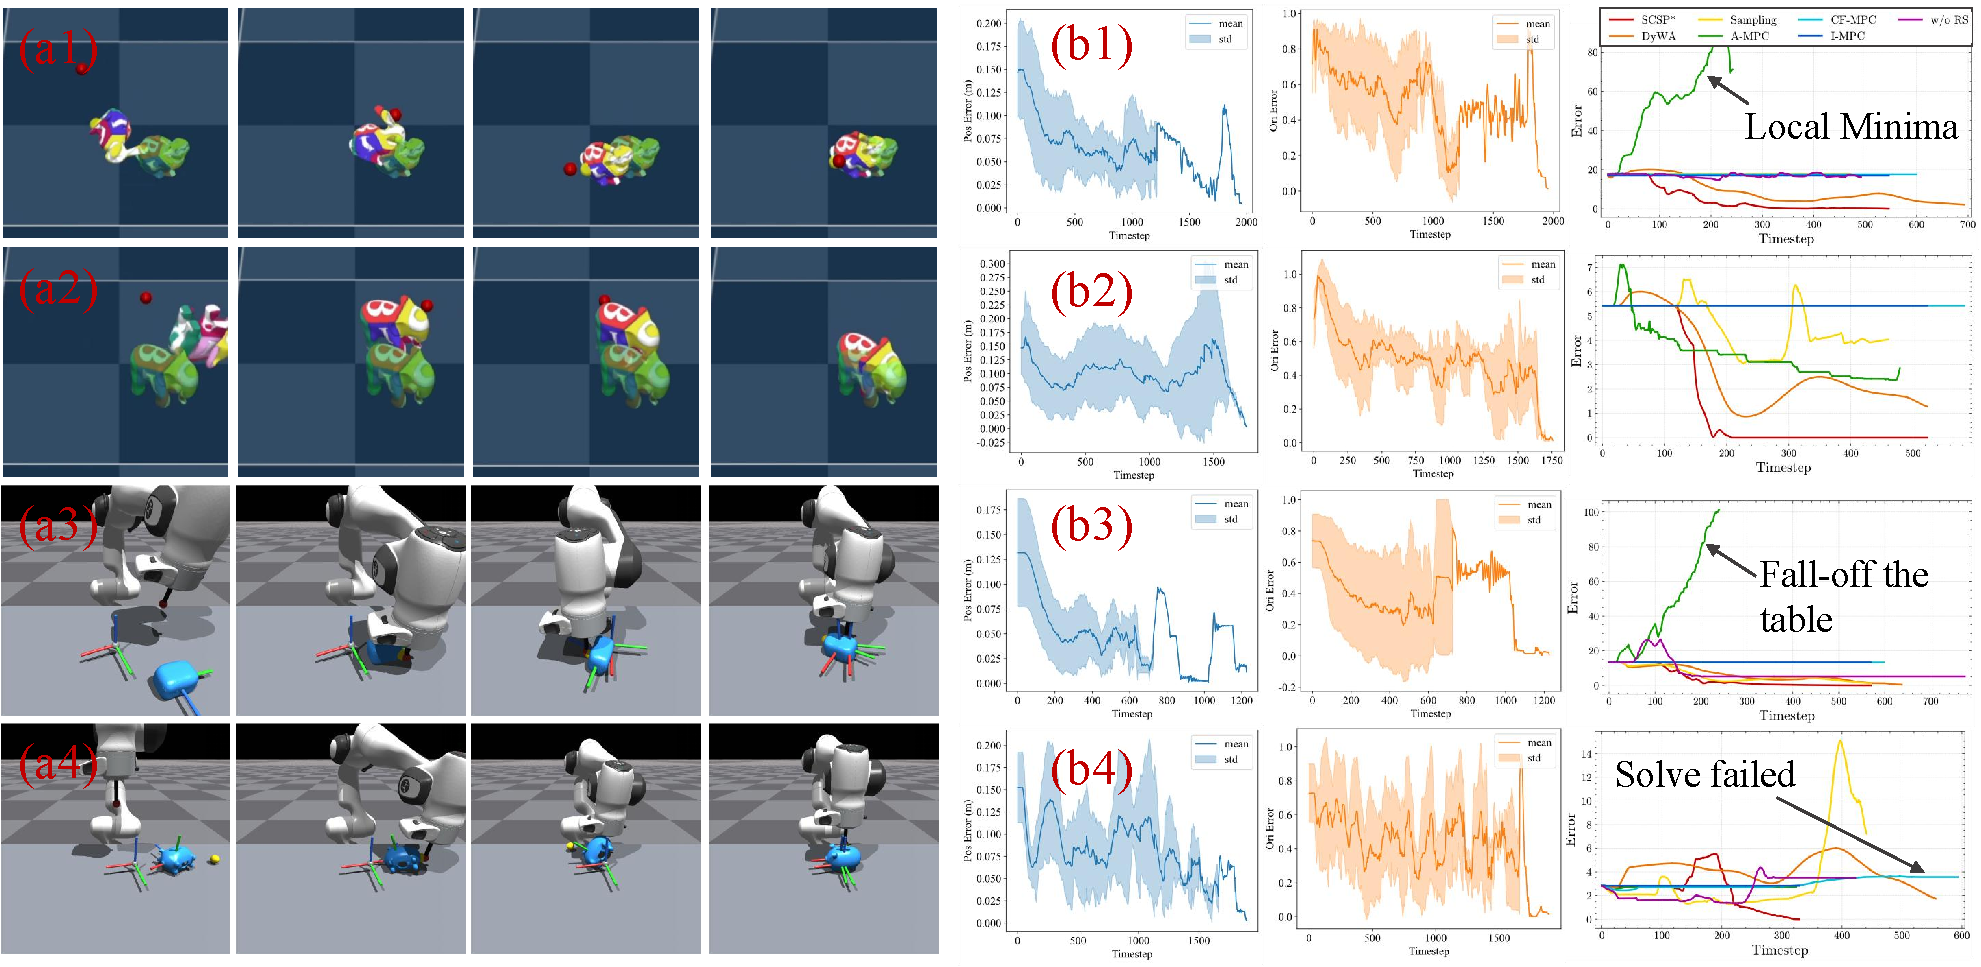
\includegraphics[width=\textwidth]{figures/exp_results.pdf}}
\caption{Nonprehensile manipulation experiments in simulation. (a1)-(a4): Snapshots of SCSP in the fingertip and robot experiments, where the goal pose is visualized either transparently or as a floating coordinate frame. (b1)-(b4): The left two panels show the mean and standard deviation curves of the position and orientation errors over steps across 10 SCSP trials. The right panel shows the pose error $\ell_{\text{pose}}$ of different methods during manipulation. The comparison methods either require longer execution time or fail due to local minima or solver failures.}\label{fig:simulation_data}
\end{figure*}

The experimental results are shown in Fig. \ref{fig:results_panda}, Fig. \ref{fig:simulation_data}, and Table \ref{tab:all_data}. SCSP achieves a higher success rate than other model-based algorithms and outperforms DyWA on all objects except the torus. Additionally, SCSP achieved the shortest execution time, demonstrating that SCSP can generate correct contact locations through CSO, thereby efficiently minimizing the pose cost of the object. SCSP also achieved the smallest convergence position error and quaternion error. Furthermore, we observed that during experiments, DyWA tends to flip objects by pressing the edges of the top surface, whereas our method makes more comprehensive decisions regarding whether to lift the object by pushing the bottom or by pressing the top. Although many flipping tasks can be accomplished through pressing, for certain objects (such as elongated objects), the pressing approach requires applying substantial torque to the object and demands sufficiently high coefficients of friction. Based on our observations, the global contact selection mechanism in CSO enables SCSP to exhibit greater diversity in its manipulation behaviors compared with other methods, rather than converging to a single strategy. 

In addition, we conducted two ablation studies. CF-MPC and A-MPC can be regarded as ablations of the contact selection strategy. CF-MPC performs contact planning without contact selection, whereas A-MPC replaces the physical reasoning of CSO-based contact planning with a simple prior. Compared with SCSP, both methods show a substantial decrease in success rate, indicating that reasonable contact selection is crucial for  complex 6D nonprehensile manipulation tasks. The w/o RS variant serves as an ablation of the ranking strategy. We observed that, since w/o RS fully follows the high-frequency output of CSO, it frequently interrupts ongoing manipulation and switches contact points, resulting in a significant drop in success rate and an increase in execution time. This suggests that it is necessary to comprehensively evaluate the contact locations produced by CSO and to balance smooth execution against the global optimality of the selected contact location.

We further validated the impact of different numbers of sampled candidate points on performance. As shown in Table \ref{tab:cso_sampling}, when the number of sampled points reaches 70, nearly the highest success rate is achieved with relatively low SCSP computation time. As the number of sampled points continues to increase, the success rate plateaus and computational efficiency deteriorates. This indicates that increasing the number of sampled points does not necessarily improve performance. There exists an optimal convergence value. For nonprehensile manipulation tasks, 70 to 100 sampled points are sufficient to characterize the geometric features of object geometries.


\begin{table}[t]
\centering
\caption{Evaluation of the effect of the number of candidate points}
\label{tab:cso_sampling}
\begin{tabular}{lccccc}
\toprule
\textbf{Sampling numbers in CSO} & \textbf{5} & \textbf{10} & \textbf{70} & \textbf{120} & \textbf{500} \\
\midrule
\textbf{Avg. Success Rate}      & 0.25  & 0.59 & \textbf{0.88} & \textbf{0.88} & 0.85 \\
\textbf{SCSP Computation Time} (s)  & \textbf{0.012} & 0.017 & 0.025 & 0.032 & 0.089 \\
\bottomrule
\end{tabular}
\end{table}


\subsection{Ablation Studies}

\subsection{Real-world Experiments}

Finally, we validate the robustness of SCSP to in real-world experiments. Most model-based methods perform well in simulation, but in real-world experiments, they often rely on highly accurate perception systems, such as motion capture. The main challenge in replacing exact perception with purely vision-based perception is that errors in pose observation can perturb contact estimation, leading to incorrect inference of contact states and consequently inaccurate contact dynamics. To the best of our knowledge, our method is the first model-based approach that can achieve purely vision-based, complex geometries, model mismatch contact-rich manipulation.

\begin{figure}[!t]
 \centerline{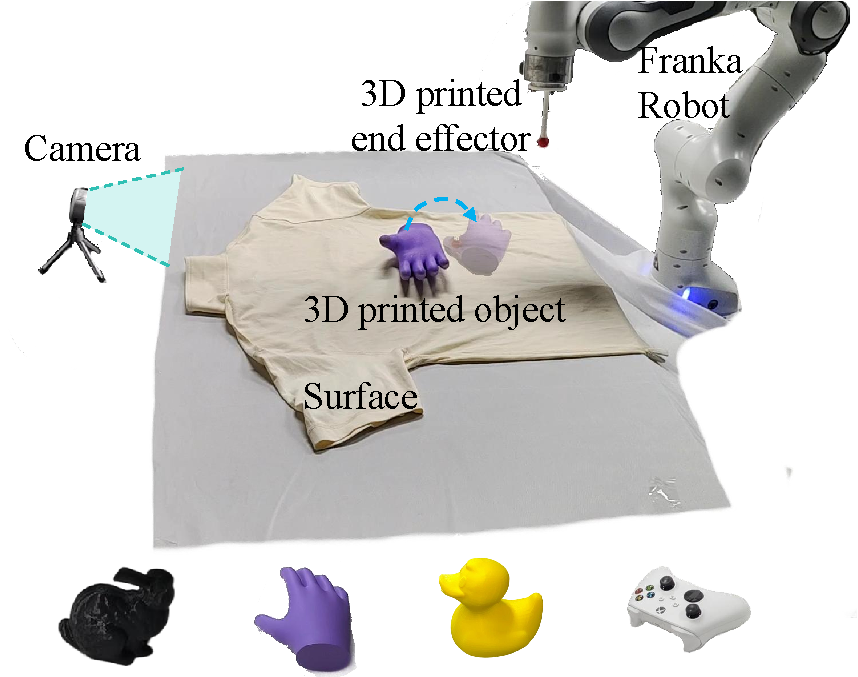
\includegraphics[width=\columnwidth]{figures/hardware_setup.pdf}}
\caption{Hardware setup of the real-world experiments.}
\label{fig:illustrative_example_1}
\end{figure}
\subsubsection{Experimental Setup}
We conduct experiments using a Franka Emika Panda equipped with a 3D-printed end-effector, and arbitrarily select 4 irregularly shaped objects: Duck, Bunny, Hand, and Xbox Controller, as shown in Fig. \ref{fig:illustrative_example_1}. We evaluate on-ground rotation on Duck and Bunny, and on-ground flipping on Bunny, Hand, and Xbox Controller. The object CAD models are obtained from the ContactDB dataset and online repositories. To validate the robustness of our method under inaccurate dynamics, we provide only rough estimates of the object’s physical parameters such as mass and friction coefficients. Moreover, instead of relying on precise motion capture for exact perception, we perform state estimation by \texttt{FoundationPose} \cite{wen2024foundationpose} using a single-view camera (Realsense D435i). In real-world experiments, precise object–environment contact locations are not directly observable. To address this, we approximately reconstruct the task environment in \texttt{MuJoCo} for contact estimation, as shown in Fig. \ref{fig:illustrative_example_i}. We perform a simple calibration procedure to determine the object’s scale parameter and positional offsets in the simulator to eliminate contact estimation misclassification. Specifically, we use Franka’s kinesthetic teaching mode to move the end-effector and make contact with several randomly selected locations on the object, and then tune the object’s scale and the offsets $[\Delta x, \Delta y, \Delta z]$ such that the simulator can approximately predict whether the end-effector is in contact with the object. The goal pose range, success conditions, and maximum execution steps for the task are identical to those in the simulation experiments. Sampling and DyWA use the same settings as in the previous section, and the outputs of DyWA are executed using an impedance controller.
\begin{figure}[!t]
 \centerline{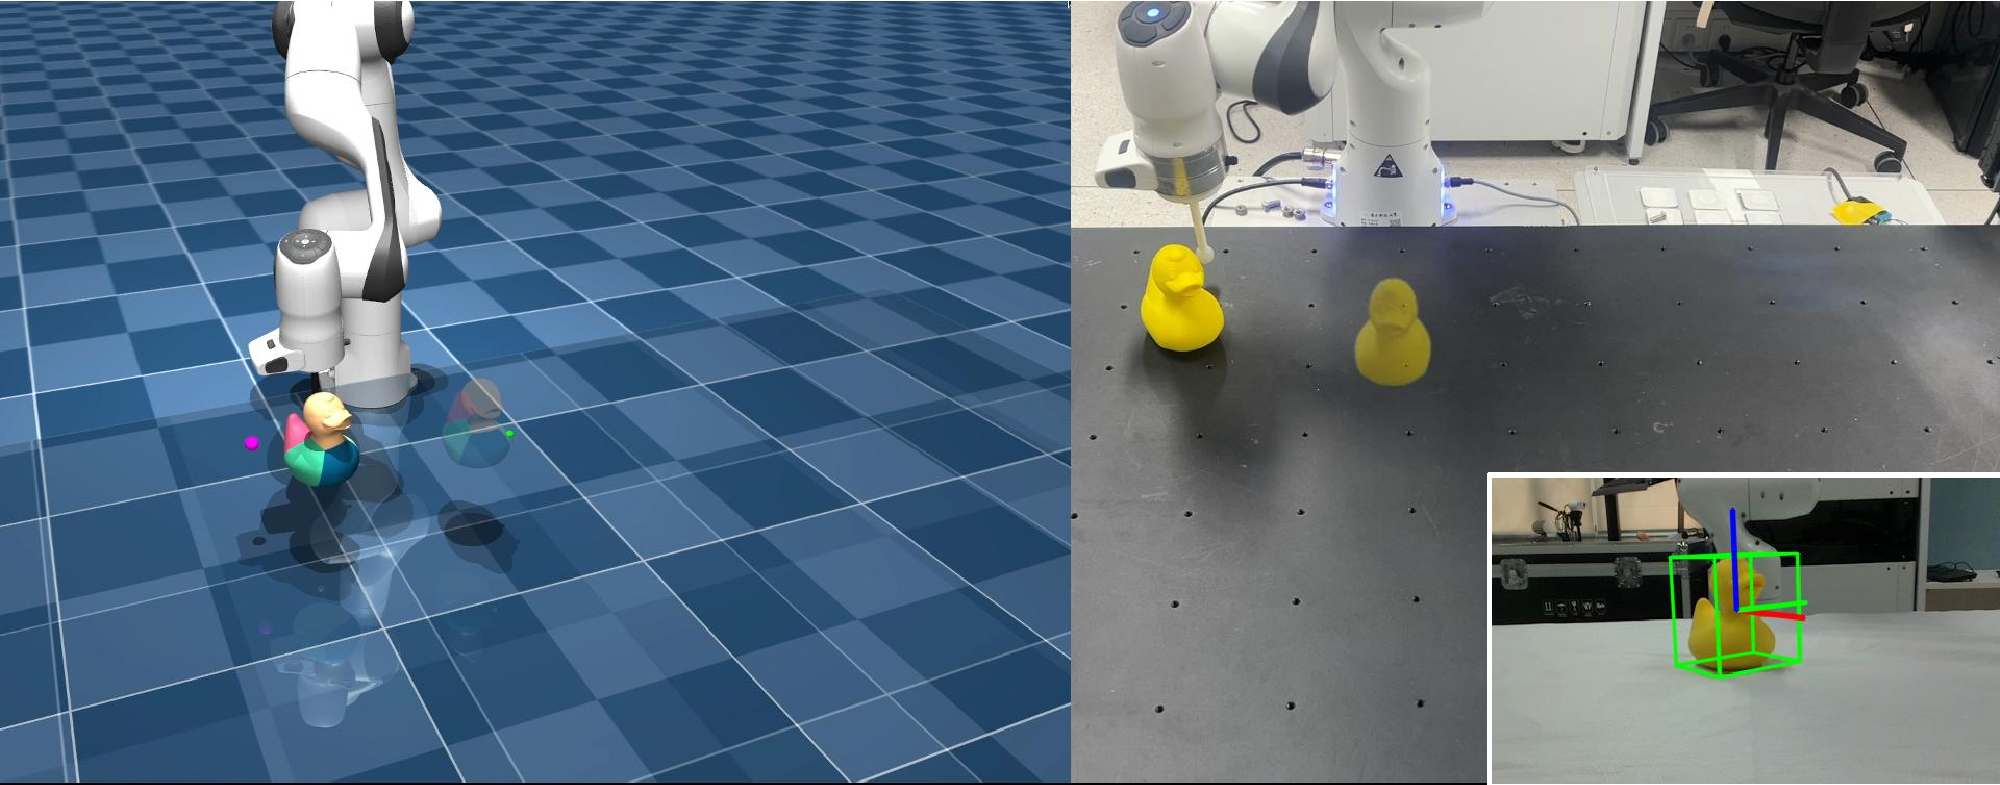
\includegraphics[width=\columnwidth]{figures/contact_sim.pdf}}
\caption{Perception method in the real-world experimental setting. Object pose is detected using \texttt{FoundationPose} and filtered via a Kalman filter. Contact estimation is performed using a \texttt{MuJoCo} implementation that approximates the experimental environment.}
\label{fig:illustrative_example_i}
\end{figure}

\begin{figure*}
 \centerline{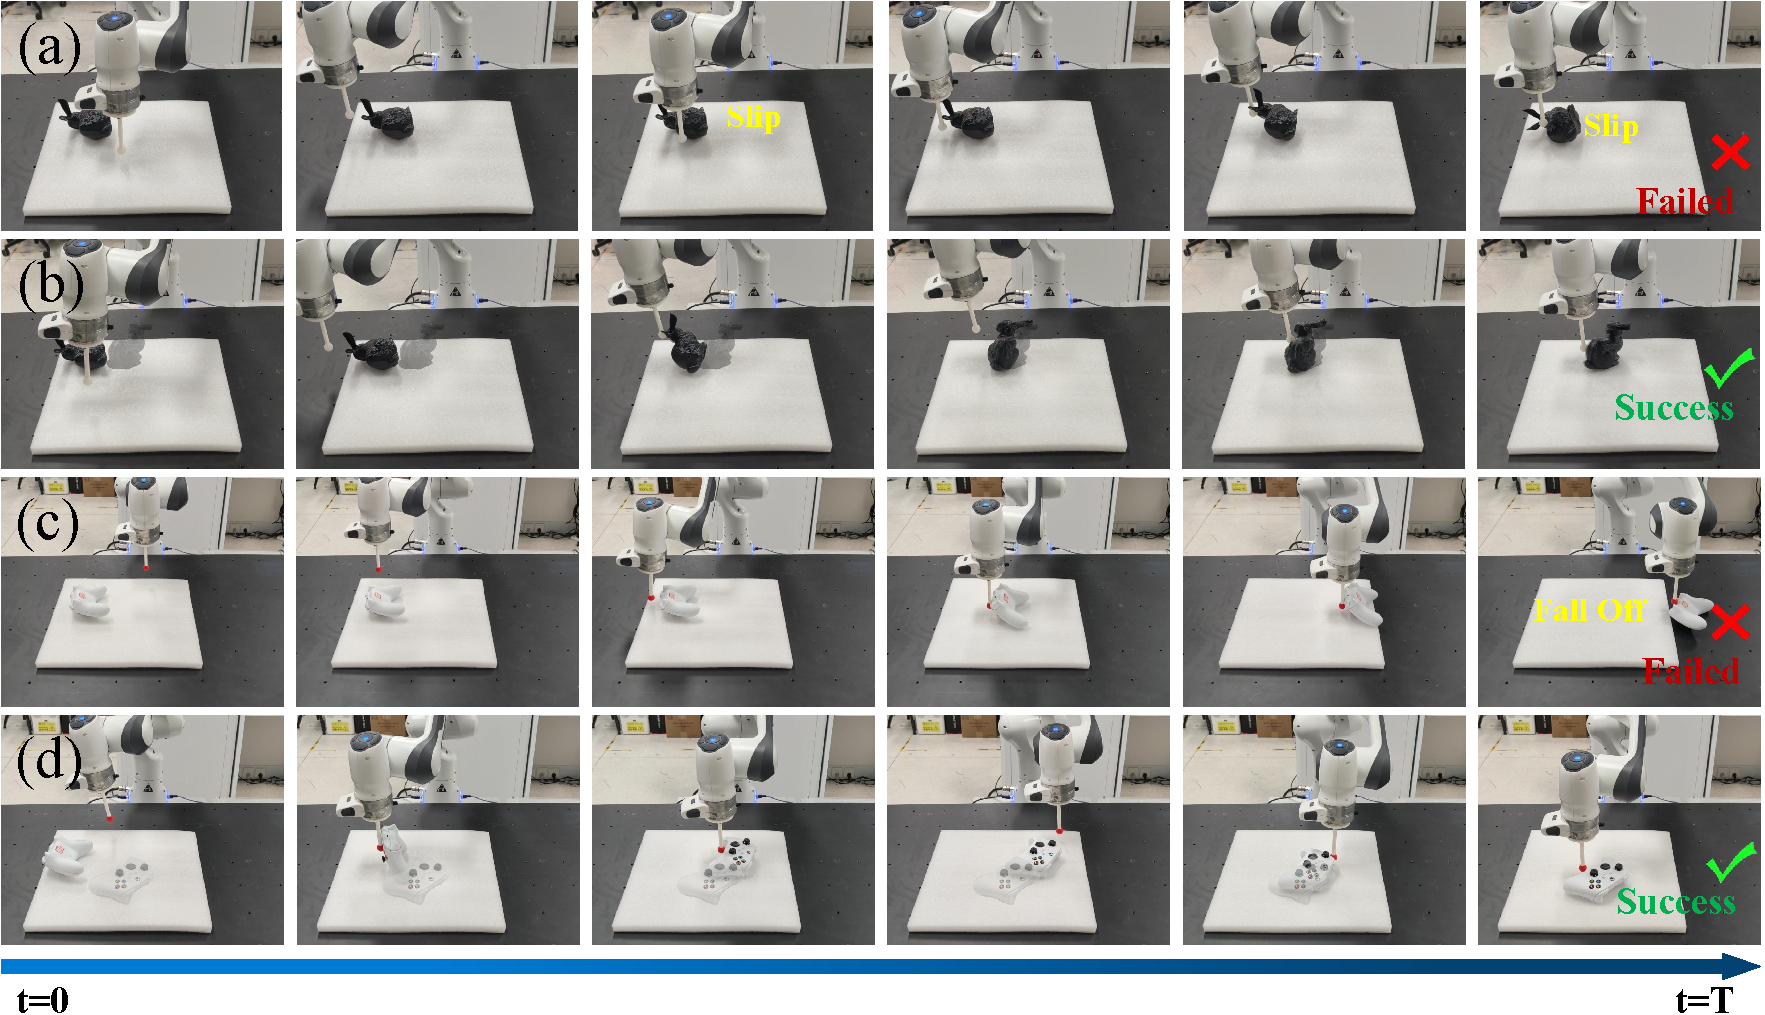
\includegraphics[width=\textwidth]{figures/real_world_exps.pdf}}
\caption{Snapshots of nonprehensile manipulation in real-world experiments. (a) \textbf{DyWA} failed to flip the bunny. (b) \textbf{SCSP} succeeds in flipping the bunny. (c) \textbf{Sampling} failed by pushing the Xbox controller to fall off the foam padding. (d) \textbf{SCSP} succeed in flipping the Xbox controller.}\label{fig:results_real_world_flip}
\end{figure*}
The OSC controller is implemented in \textsf{c++}. Unlike in simulation experiments, control in real-world deployment is subject to disturbances, leading to control lag and steady-state errors. To address this, we designed an adaptive controller for precise control, which we refer to as the Incremental OSC. We introduce an intermediate position vector $\boldsymbol{p}_{\text{inc}} = \boldsymbol{p}_{\text{inc}} + \boldsymbol{K}_{\text{inc}}\boldsymbol{u}$,
and replace $\boldsymbol{e}_{\text{pos}}$  with $\boldsymbol{e}_{\text{pos}}=\boldsymbol{p}_{\text{inc}}-\boldsymbol{p}_{\text{ee}}$. The steady-state error is adaptively eliminated under the high-frequency self-integrating effect. In the experiment, we set
$\boldsymbol{K}_{\text{inc}}=0.01 \boldsymbol{I}_3$, $\boldsymbol{K}_x = \text{diag}(500,500,500,10,10,10)$ and $\boldsymbol{D}_x = \sqrt{2\boldsymbol{K}_x}$.

\subsubsection{Results and Discussion}

\begin{table*}[t]
\centering
\caption{Success rates (\%) for on-ground rotation and flipping on different surfaces and objects.}
\label{tab:real_world_success}
\setlength{\tabcolsep}{5pt}
\begin{tabular*}{\textwidth}{@{\extracolsep{\fill}} lcccccccccc}
\toprule
& \multicolumn{4}{c}{\textbf{On-ground rotation}}
& \multicolumn{6}{c}{\textbf{On-ground flipping}} \\
\cmidrule(lr){2-5} \cmidrule(lr){6-11}
\textbf{Method}
& \multicolumn{2}{c}{Duck}
& \multicolumn{2}{c}{Bunny}
& \multicolumn{2}{c}{Bunny}
& \multicolumn{2}{c}{Hand}
& \multicolumn{2}{c}{Xbox} \\
\cmidrule(lr){2-3} \cmidrule(lr){4-5}
\cmidrule(lr){6-7} \cmidrule(lr){8-9} \cmidrule(lr){10-11}
& Smooth & Rough
& Smooth & Rough
& Smooth & Rough
& Smooth & Rough
& Smooth & Rough \\
\midrule
Sampling
& 9 / 20 & 5 / 20
& 7 / 20 & 4 / 20
& 0 / 20 & 0 / 20
& 0 / 20 & 0 / 20
& 0 / 20 & 0 / 20 \\
DyWA
& 6 / 20 & 4 / 20
& 2 / 20 & 1 / 20
& 0 / 20 & 0 / 20
& 0 / 20 & 0 / 20
& 0 / 20 & 0 / 20 \\
SCSP*
& \textbf{20 / 20} & \textbf{19 / 20}
& \textbf{5 / 20} & \textbf{5 / 20}
& \textbf{2 / 20} & \textbf{3 / 20}
& \textbf{3 / 20} & \textbf{4 / 20}
& \textbf{4 / 20} & \textbf{5 / 20}\\
\bottomrule
\end{tabular*}
\end{table*}

We first evaluate the success rate of SCSP across different objects and tabletop materials to assess its robustness under model inaccuracies. The experimental results are shown in Fig. \ref{fig:results_real_world_flip}, \ref{fig:real_world_continous} and Table \ref{tab:real_world_success}. They indicate that our method maintains strong performance even under perception noise and model mismatch.

We conducted each experiment on two different tabletop materials: smooth and rough as in Fig. \ref{fig:real_world_disturbance}. For the on-ground rotation experiments, the smooth surface denotes a tabletop with low friction, whereas the rough surface denotes cotton clothes. For the on-ground flipping experiments, which require greater friction, we use foam padding as the rough surface and cotton cloth as the smooth surface. Note that our method does not measure friction coefficients, object mass, or other physical parameters, but instead uses coarse estimates. Additionally, biases in contact estimation and noise in object pose estimation can interfere with the decision-making of SCSP. The experiment results suggest that SCSP can effectively cope with model inaccuracies and disturbances, which is typically challenging for model-based methods. 

As shown in Table \ref{tab:real_world_success}, SCSP achieved a 100\% success rate in the on-ground rotation experiments with complex object geometries and also showed strong performance in the flipping tasks, whereas the comparison methods failed in nearly all flipping experiments. We observe that the failures of DyWA mainly arose from contact slippage and violations of the Franka acceleration limits during pressing, while the failures of Sampling were primarily caused by the selection of unstable contact locations. Due to the complex geometry and relatively smooth material of the 3D printed objects, the fingertip sometimes fails to establish stable contact with the object, resulting in relative sliding that causes the execution of the contact plan planned by SCSP to fail. Additionally, surface friction also affects the success rate of flipping. As shown in the results, SCSP achieves a notably higher success rate on the rough surface compared with the smooth surface.

We further conduct continuous manipulation experiments, as shown in Fig. \ref{fig:real_world_continous}. During manipulation, we repeatedly perturb the object pose to evaluate the real-time performance, closed-loop planning capability, and robustness of SCSP under accumulated perception errors. Under repeated perturbations, both the pose estimated from \texttt{FoundationPose} and the contact estimation become biased. However, SCSP exhibits strong replanning capability and consistently completes the continuous manipulation tasks under disturbances.

We combine the preceding experimental results to analyze the source of SCSP’s robustness to model mismatch. We conclude that: 1) the ablation study reveals that optimality of the contact prior is not necessary. Although the prior is important for contact planning, even a coarse contact location selection as a prior can still bring substantial performance improvement. This observation also provides insight into the role of the contact-selection model: how to properly connect the prior with the planning framework seems to be more important than the optimality and accuracy of the prior itself. The designs of CSO and the ranking strategy are both developed with this perspective. 2) CPO has a strong closed-loop nature. The real-time performance and robustness of CIMPC methods have been thoroughly validated in previous work. CPO is a prior-guided contact planning framework built upon the CIMPC formulation. It inherits the robustness of CIMPC while improving manipulation diversity. Therefore, the SCSP framework is able to achieve robust performance.

\begin{table}[t]
\centering
\caption{Computation time of SCSP}
\label{tab:metrics}
\begin{tabular*}{0.8\columnwidth}{@{\extracolsep{\fill}} l c}
\toprule
\textbf{Metric} & \textbf{Value} \\
\midrule
\multicolumn{2}{c}{\textbf{CSO Computation time}} \\
\midrule
\textcolor{red}{Offline sampling cost time} (s)           & $4.82 \pm 3.85$ \\
Exchange cost time (ms)          & $0.002 \pm 0.01$ \\
MIQP cost time (ms)              & $0.23 \pm 0.01$ \\
CSO solving time (ms)            & $16.21 \pm 0.58$ \\
\midrule
\multicolumn{2}{c}{\textbf{CPO Computation time}} \\
\midrule
RS cost time (s)                 & $0.01 \pm 0.00$ \\
Average CPO solving time (ms)  & $8.68 \pm 0.31$ \\
\bottomrule
\end{tabular*}
\end{table}



\begin{figure*}
 \centerline{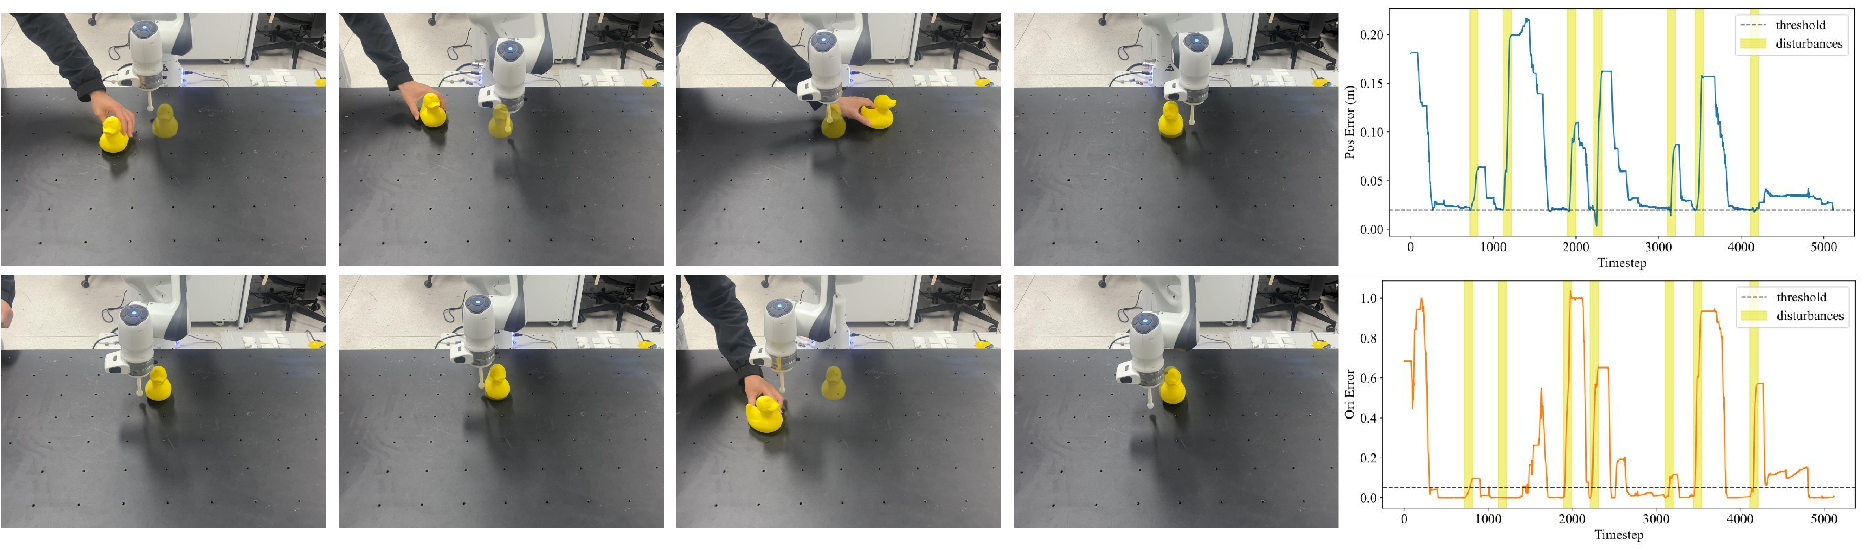
\includegraphics[width=\textwidth]{figures/consecutive_manipulation.pdf}}
\caption{Snapshots of manipulation under external disturbances. The object’s pose is continuously perturbed during manipulation to demonstrate SCSP’s real-time robustness under such disturbances. The panels on the right shows the temporal evolution of position and orientation errors.}\label{fig:real_world_continous}
\end{figure*}


\begin{figure}
 \centerline{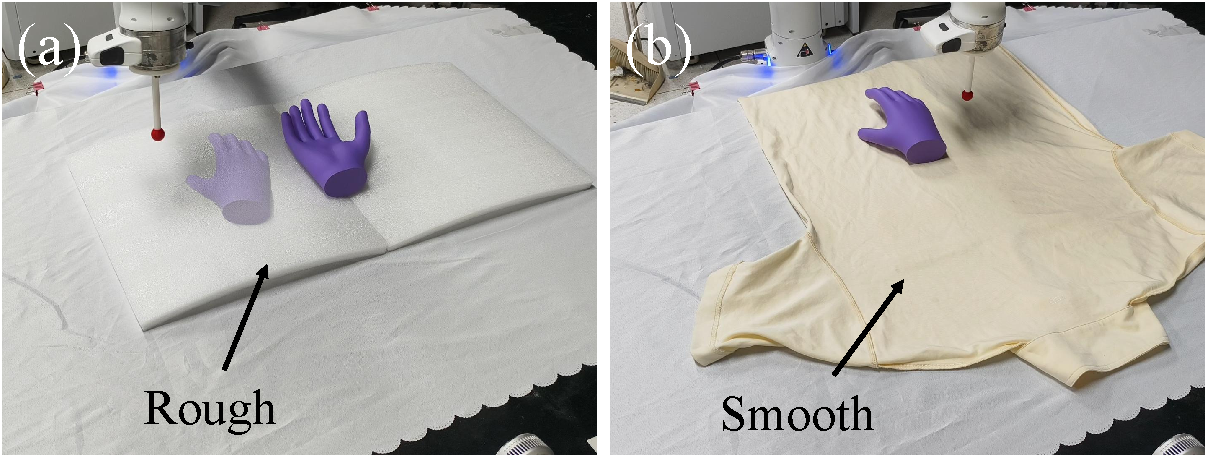
\includegraphics[width=\columnwidth]{figures/real_world_2.pdf}}
\caption{Robustness validation of SCSP on surfaces with different friction. (a) Foam. (b) Cotton clothes.}\label{fig:real_world_disturbance}
\end{figure}










